\documentclass{article}
\usepackage[utf8]{inputenc}
\usepackage{fullpage}
\usepackage{amsmath}
\usepackage{caption}
\usepackage{subcaption}
\captionsetup[subfigure]{justification=raggedright,singlelinecheck=false}
\usepackage{graphicx}
\usepackage{pgfplots}
\pgfplotsset{compat=1.9}
\usepackage{biblatex}
\addbibresource{citations.bib}

\title{The Paradox of the Perfect Spiral}
\author{Tyler Lin}
\date{May 2021}

\begin{document}

\maketitle

\section{Introduction}
Any fan of the NFL can appreciate the beauty of a perfect spiral pass. We've seen it time and time again: a quarterback steps forward, cocks the ball back, and launches a deep pass off their fingertips. The ball points upwards immediately after release, but as the ball sails through the air, the nose gradually dips downwards before landing right in the hands of the receiver.

\begin{figure}[h]
     \begin{subfigure}[b]{0.3\textwidth}
         \includegraphics[width=\textwidth]{img/throw.png}
         \caption{The ball is released at an upwards angle.}
     \end{subfigure}
     \hfill
     \begin{subfigure}[b]{0.3\textwidth}
         \includegraphics[width=\textwidth]{img/peak.png}
         \caption{The ball is straight at the peak of its flight.}
     \end{subfigure}
     \hfill
     \begin{subfigure}[b]{0.3\textwidth}
         \includegraphics[width=\textwidth]{img/catch.png}
         \caption{The ball ends at a downward angle.}
     \end{subfigure}
    \caption{A perfect spiral thrown by quarterback Baker Mayfield.}
    \label{bakerspiral}
\end{figure}

The longitudinal axis of the football remains tangent to the football's velocity throughout its flight, a quirk that football fans and players often take for granted. It makes sense that the angle of the ball would follow its trajectory to reduce drag. However, there's just one problem. The law of conservation of angular momentum in physics states that the angular momentum of an object remains constant when no net external torque acts upon it. In other words, the longitudinal axis of a spinning object maintains its orientation unless torque causes it to move. Torque is a measure of the force that causes an object to rotate. Think of a door: when you push a door open, you apply torque by rotating it around its hinges. 

Conservation of angular momentum is made evident by the example of a spinning top. A spinning top continues to spin because its angular momentum points up and remains constant due to the lack of external torque affecting the top's rotation. It's important to note that the force of gravity does not cause torque, because it's applied to the center of the top and doesn't affect its rotation. Over time, though, the dissipative force of friction causes enough external torque for the top to become unbalanced and topple.

In the case of a spiraling football, there's no friction to cause torque on the ball. Gravity again acts equally on all parts of the ball, so it doesn't cause torque either. Therefore, the nose of the ball should point upwards throughout its entire arc by conservation of angular momentum. So why does it dip?

\subsection{Air Resistance}
If neither gravity nor friction can explain this phenomenon, there's only one possibility left: air resistance. In physics class, the effect of air resistance is often so negligible that we completely ignore it. But could it be what causes a spiraling football to orient itself with its trajectory?

When you envision a spiral, it seems as if air resistance would have the exact opposite effect: the air would push against the nose of the ball and rotate it backwards against its trajectory. We must employ a more careful mathematical approach to determine exactly how air resistance causes a perfect spiral to maintain tangency with its trajectory.

\section{Setup}
We will represent the flight of a spiral pass in $xyz$ space such that the football's trajectory begins on the negative $x$ axis, intersects the positive $y$ axis, and ends on the positive $x$ axis, per figure \ref{space} The $z$ axis is perpendicular to the plane of the page.

\begin{figure}[h]
\centering
    \includegraphics[width=0.5\textwidth]{img/space.png}
    \caption{Our chosen coordinate system geometry. The ball travels within the $xy$ plane and rotates clockwise from the perspective of the quarterback.}
    \label{space}
\end{figure}

We must consider the ball's velocity $\mathbf{v}$ and the direction $\mathbf{\hat{d}}$ of its longitudinal axis. The spiral of the ball itself is also a factor in its flight, so we will consider the ball's angular momentum $\mathbf{L}$.

Given that the ball is thrown straight, $\mathbf{v}$ and $\mathbf{\hat{d}}$ are both vectors in the $xy$ plane. To determine the direction of $\mathbf{L}$, we use the formula
\begin{equation}
    \mathbf{L} = \mathbf{r} \times \mathbf{p} \text{,}
\end{equation}
where $\mathbf{r}$ represents the position of a point on the object relative to the center of mass, and $\mathbf{p}$ represents the linear momentum at that point. For a right-handed quarterback, the ball spirals clockwise, so we can determine using the right-hand rule that $\mathbf{L}$ also points along the $xy$ plane in the direction of $+y$.

\begin{figure}[h]
\centering
    \includegraphics[width=0.75\textwidth]{img/vectors.png}
    \caption{The relevant vectors in our investigation of the flight of a spiraling football.}
    \label{vectors}
\end{figure}

Because $\mathbf{L}$ is perpendicular to $\mathbf{r}$ and $\mathbf{r}$ is perpendicular to $\mathbf{\hat{d}}$ in the $xy$ plane, we can conclude that $\mathbf{L}$ is colinear with $\mathbf{\hat{d}}$, which means that the angle between them is $0$. Therefore, we can set
\begin{equation}\label{L}
    \mathbf{L} = L\mathbf{\hat{d}}\text{,}
\end{equation}
where $L$ is the magnitude of $\mathbf{L}$.

In a truly "perfect" spiral, $\mathbf{v}$ would also be colinear with $\mathbf{L}$ and $\mathbf{\hat{d}}$; however, this is not realistic. As shown in figure \ref{vectors}, $\mathbf{v}$ may not be aligned with $\mathbf{\hat{d}}$. This is the key to our problem. If you watch slow-motion video of deep balls, you will notice that every pass wobbles, even if only just a tiny bit. Not even Tom Brady can throw a perfectly tight spiral that doesn't wobble! 

Why is wobble important? The force due to air resistance is given by
\begin{equation}\label{drag}
    \mathbf{F}_{\text{air}} = -\frac{1}{2}\rho AC|\mathbf{v}|^2\mathbf{\hat{v}}\text{,}
\end{equation}
where $\rho$ is the density of air, $A$ is the cross-sectional area of the object, and $C$ is the drag coefficient of the object. Equation \ref{drag} tells us that $\mathbf{F}_{\text{air}}$ and $\mathbf{v}$ are colinear and opposite. Without wobble, $\mathbf{F}_{\text{air}}$ and $\mathbf{\hat{d}}$ would then also be colinear and opposite, so $\mathbf{F}_{\text{air}}$ should cause no torque on the ball. Indeed, we can prove this using the definition of torque
\begin{equation}\label{torque}
    \pmb{\tau} = \mathbf{r} \times \mathbf{F}\text{.}
\end{equation}
In our case, $\mathbf{r} = \ell\mathbf{\hat{d}}$, where $\ell$ is the length from the football's center of mass to its nose, and $\mathbf{F} = \mathbf{F}_{\text{air}}$. Therefore,
\begin{equation}\label{airtorque1}
    \begin{split}
        \pmb{\tau}_{\text{air}} &= \ell\mathbf{\hat{d}} \times \mathbf{F}_{\text{air}} \\
        &= \ell \cdot -\frac{1}{2}\ell\rho AC|\mathbf{v}|^2(\mathbf{\hat{d}} \times \mathbf{\hat{v}}) \propto \sin{(\theta)} \\
        &= \frac{1}{2}\ell\rho AC|\mathbf{v}|^2(\mathbf{\hat{v}} \times \mathbf{\hat{d}}) \propto \sin{(\theta)} \\
        &= \kappa(\mathbf{\hat{v}} \times \mathbf{\hat{d}}) \propto \sin{(\theta)}\text{,}
    \end{split}
\end{equation}
where $\theta$ is the angle between $\mathbf{\hat{d}}$ and $\mathbf{v}$ and
\begin{equation}
    \kappa = \frac{1}{2}\ell\rho AC|\mathbf{v}|^2\text{.}
\end{equation}
Note that $\pmb{\tau}_{\text{air}}$ points in the direction of the cross product of $\mathbf{\hat{v}}$ and $\mathbf{\hat{d}}$. As shown in figure \ref{vectors}, $\pmb{\tau}_{\text{air}}$ initially points in the positive $z$ direction due to the right-hand rule. From equation \ref{airtorque1} it is easy to tell that $\pmb{\tau}_{\text{air}} = 0$ when $\theta = 0$, or when there is no wobble.

When the ball does wobble, the direction of $\mathbf{\hat{d}}$ deviates from the direction of $\mathbf{v}$, so $\theta > 0$ and $\pmb{\tau}_{\text{air}} > 0$. The issue, however, is that when $\theta = \pi/2$, $\pmb{\tau}_{\text{air}} = -\kappa\mathbf{\hat{z}}$ when it should, in theory, equal $0$ because $\mathbf{F}_{\text{air}}$ would occur at the base of the ball perpendicular to $\mathbf{\hat{d}}$. Imagine a football falling straight down with its longitudinal axis parallel to the ground; air resistance would have no effect on the ball's tilt. To resolve this, we simply halve the period of $\pmb{\tau}_{\text{air}}$, giving
\begin{equation}\label{airtorque2}
    \pmb{\tau}_{\text{air}} = \kappa(\mathbf{\hat{v}} \times \mathbf{\hat{d}}) \propto \sin{(2\theta)}\text{.}
\end{equation}
Now, $\pmb{\tau}_{\text{air}} = 0$ at $\theta = \pi/2$ as desired.

The angle of wobble in a well-thrown spiral is small, so we can apply the small-angle approximation $\sin{\theta}=\theta$ to equation \ref{airtorque2} to produce a final equation
\begin{equation}\label{airtorque3}
    \pmb{\tau}_{\text{air}} = 2\kappa(\mathbf{\hat{v}} \times \mathbf{\hat{d}}) \propto \theta \text{.}
\end{equation}

Because we are primarily concerned with the behavior of $\mathbf{\hat{d}}$ in relation to $\mathbf{v}$, we assume that $\mathbf{v}$ follows a fixed parabolic path per the rules of projectile motion and is not affected by air resistance, allowing us to focus solely on $\pmb{\tau}_{\text{air}}$ and its effect.

\section{Visualization}
Before we conduct any calculations, we should first try to predict intuitively how the torque due to air resistance will affect the ball.

At the time the ball is released from the quarterback's hand, $\mathbf{\hat{d}}$, $\mathbf{L}$, and $\mathbf{v}$ are aligned. Immediately after launch, the force of gravity would cause $\mathbf{v}$ to tilt downwards, which separates it from $\mathbf{\hat{d}}$ and causes a torque in the $+z$ direction as shown in figure \ref{precession1}.

By the rotational equivalent of Newton's second law (we will use Newton's over-dot notation to denote a time derivative),
\begin{equation}\label{secondlaw}
    \frac{\mathbf{dL}}{dt} = \mathbf{\dot{L}} = \pmb{\tau}\text{.}
\end{equation}
Therefore, the torque causes a change in the ball's angular momentum in the $+z$ direction. Equation \ref{L} tells us that $\mathbf{L}$ is aligned with $\mathbf{\hat{d}}$, so $\mathbf{\hat{d}}$ is also transformed in the $+z$ direction. In other words, the nose tilts to the right from the quarterback's point of view, or to the left from the receiver's point of view as shown in figure \ref{precession2}.

Let's quickly define a couple of terms commonly used in the field of aerospace to make this explanation easier. \textbf{Yaw} is the rotation of the football about its $y$ axis that changes the direction it is pointing to the left or right of its direction of velocity. \textbf{Pitch} is the rotation of the football about its $z$ axis that raises or lowers its nose. As such, the torque in the $+z$ direction causes the ball to "yaw right".

\begin{figure}[h]
     \begin{subfigure}[b]{0.3\textwidth}
         \includegraphics[width=\textwidth]{img/precession (1).png}
         \caption{$\mathbf{v}$ points at a higher angle than $\mathbf{\hat{d}}$, creating a torque $\pmb{\tau}$ in the $+z$ direction.}
         \label{precession1}
     \end{subfigure}
     \hfill
     \begin{subfigure}[b]{0.3\textwidth}
         \includegraphics[width=\textwidth]{img/precession (2).png}
         \caption{$\pmb{\tau}$ causes $\mathbf{\hat{d}}$ to deviate in the $+z$ direction, in turn causing $\pmb{\tau}$ to deviate in the $-y$ direction.}
         \label{precession2}
     \end{subfigure}
     \hfill
     \begin{subfigure}[b]{0.3\textwidth}
         \includegraphics[width=\textwidth]{img/precession (3).png}
         \caption{$\pmb{\tau}$ causes $\mathbf{\hat{d}}$ to deviate in the $-y$ direction, in turn causing $\pmb{\tau}$ to deviate in the $-z$ direction.}
         \label{precession3}
     \end{subfigure}
    \caption{The predicted behaviors of $\mathbf{\hat{d}}$, $\mathbf{v}$, and $\pmb{\tau}$ during a tight spiral pass, as shown from the reciever's point of view (looking in the $-x$ direction). $\mathbf{\hat{d}}$ and $\pmb{\tau}$ move in generally circular paths, while $\mathbf{v}$ constantly rotates downward due to gravity.}
    \label{precession}
\end{figure}

Because $\mathbf{\hat{d}}$ now has a component in the the $+z$ direction, the torque develops a component in the $-y$ direction by the right-hand rule, as shown in figure \ref{precession2}. Consequently, the ball pitches downwards, creating a component of torque in the $-z$ direction again by the right-hand rule, as shown in figure \ref{precession3}. This new torque will alter the ball's yaw, which will alter the torque, which will alter the ball's pitch, and so on. This cycle of interaction between torque and $\mathbf{\hat{d}}$ is analogous to the relationship between velocity and centripetal acceleration, so we can infer that $\mathbf{\hat{d}}$, and equivalently the nose of the football, moves in an approximately circular path within the $yz$ plane. Indeed, this is a common behavior in spinning objects known as \textbf{gyroscopic precession}.

A gyroscope is a spinning object, such as a top, whose axis of rotation is free to assume any orientation. Precession is a change in the orientation of the axis of rotation. Gyroscopic precession describes how a gyroscope precesses, which we can imagine using the example of a top. If you place a top at an angle on a flat surface without spinning it, it will fall over due to the torque caused by gravity, as shown in figure \ref{top1}. If the top is spinning, however, it will have an angular momentum $\mathbf{L}$ pointing upwards in the axis of rotation, as shown in figure \ref{top2}. The torque will then cause a change in $\mathbf{L}$ according to equation \ref{secondlaw}. Because the torque is always horizontal and perpendicular to $\mathbf{L}$, the top precesses about the $y$ axis, and the tip follows the circular dotted path. In the case of a spiral pass, the torque is always perpendicular to $\mathbf{L}$, so the nose precesses about some axis.

\begin{figure}[h]
    \hspace*{\fill}
     \begin{subfigure}[t]{0.4\textwidth}
         \includegraphics[width=\textwidth]{img/top (1).png}
         \caption{When the top is not spinning, the torque due to gravity $\pmb{\tau_g}$ causes the top to fall over.}
         \label{top1}
     \end{subfigure}
     \hfill
     \begin{subfigure}[t]{0.4\textwidth}
         \includegraphics[width=\textwidth]{img/top (2).png}
         \caption{When the top is spinning, $\pmb{\tau_g}$ causes a change $\mathbf{dL}$ in the top's angular momentum $\mathbf{L}$, and the top precesses about the $y$ axis.}
         \label{top2}
     \end{subfigure}
     \hspace*{\fill}
    \caption{A comparison of the rotational motion of an idle top and a spinning top, both at an angle to the vertical.}
\end{figure}

Gyroscopic precession explains how torque due to air resistance can affect the pitch of a spiraling football.

Figure \ref{precession} also illustrates how $\mathbf{v}$ slowly rotates downwards due to gravity throughout this flight. Knowing that $\mathbf{\hat{d}}$ maintains general tangency with the trajectory of the ball, we can predict that the ball precesses relative to $\mathbf{v}$ rather than some fixed point. Now, we must do the math to determine the exact nature in which the nose moves.

\section{Calculations}
We start by trying to find the rate $\omega_p$ at which the ball gyroscopically precesses. From equation \ref{airtorque3}, $|\pmb{\tau}_{\text{air}}| = \tau_{\text{air}} = 2\kappa\theta$.
Substituting into equation \ref{secondlaw} and multiplying by $dt$ gives us
\begin{equation*}
    dL = 2\kappa\theta dt\text{.}
\end{equation*}
The radius of the dotted circle in figure \ref{top2} is $L\sin{\theta}$, which simplifies to $L\theta$ by the small-angle approximation. Thus, the angle $\phi$ that the ball precesses through in time $dt$ is
\begin{equation*}
    d\phi = \frac{dL}{L\theta} = \frac{2\kappa\theta}{L\theta}dt = \frac{2\kappa}{L}dt\text{.}
\end{equation*}
The angular velocity of precession would be $\frac{d\phi}{dt}$, so we divide by $dt$ to finish with
\begin{equation}\label{omega}
    \omega_p = \frac{d\phi}{dt} = \frac{2\kappa}{L}\text{.}
\end{equation}

We can now use equation \ref{omega} to model the movement of $\mathbf{\hat{d}}$ over time. Substituting equation \ref{airtorque3} into equation \ref{secondlaw},
\begin{equation}\label{Lair}
    \mathbf{\dot{L}} = 2\kappa(\mathbf{\hat{v}} \times \mathbf{\hat{d}})\text{.}
\end{equation}
$\mathbf{L} = L\mathbf{\hat{d}}$ from equation \ref{L}, so we substitute into the left-hand side to get
\begin{equation*}
    L\mathbf{\dot{\hat{d}}} = 2\kappa(\mathbf{\hat{v}} \times \mathbf{\hat{d}})\text{.}
\end{equation*}
We keep $L$ outside of the derivative because we know from the previous section that precession does not change the magnitude of $\mathbf{L}$, only its direction. This allows us to divide both sides by $L$, so equation \ref{Lair} becomes
\begin{equation}\label{dair}
    \mathbf{\dot{\hat{d}}} = \frac{2\kappa}{L}(\mathbf{\hat{v}} \times \mathbf{\hat{d}}) = \omega_p(\mathbf{\hat{v}} \times \mathbf{\hat{d}})\text{.}
\end{equation}

Still, we are concerned not with how $\mathbf{\hat{d}}$ behaves by itself, but with how $\mathbf{\hat{d}}$ behaves relative to $\mathbf{\hat{v}}$. To obtain insight into the manner in which $\mathbf{\hat{d}}$ deviates from $\mathbf{\hat{v}}$, we consider the projection $\mathbf{P}$ of $\mathbf{\hat{d}}$ onto a plane perpendicular to $\mathbf{\hat{v}}$. This plane shall be specified by the coordinate system $(\mathbf{\hat{X}}, \mathbf{\hat{Y}})$ defined by $(\mathbf{\hat{z}}, \mathbf{\hat{z}} \times \mathbf{\hat{v}})$, as illustrated in figure \ref{projection}. Thus, we define $\mathbf{P}$ as
\begin{equation}
    \mathbf{P} = P_X \mathbf{\hat{X}} + P_Y \mathbf{\hat{Y}}\text{,}
\end{equation}
where we can think of $P_X$ as the ball's yaw and $P_Y$ as the ball's pitch.

\begin{figure}[h]
\centering
    \includegraphics[width=0.5\textwidth]{img/projection.png}
    \caption{An illustration of our projection plane (in yellow), made up by the $\mathbf{\hat{X}}$ and $\mathbf{\hat{Y}}$ axes. By definition, $\mathbf{\hat{X}}$ is parallel to the $z$ axis and $\mathbf{\hat{Y}}$ is perpendicular to both the $z$ axis and $\mathbf{v}$. Vector $\mathbf{P} = \langle P_X, P_Y \rangle$ (in green) is the projection of $\mathbf{\hat{d}}$ onto our plane.}
    \label{projection}
\end{figure}

To determine $P_X$, we must calculate the magnitude of the vector projection of $\mathbf{\hat{d}}$ onto $\mathbf{\hat{X}}$:
\begin{equation}\label{P_X}
    \begin{split}
        P_X &= |proj_{\mathbf{\hat{X}}}\mathbf{\hat{d}}| \\
        &= \mathbf{\hat{d}} \boldsymbol{\cdot} \mathbf{\hat{X}} \\
        &= \mathbf{\hat{d}} \boldsymbol{\cdot} \mathbf{\hat{z}} \\
        &= \langle \hat{d}_x,\hat{d}_y,\hat{d}_z \rangle \boldsymbol{\cdot} \langle 0,0,1 \rangle \\
        &= \hat{d}_z\text{.}
    \end{split}
\end{equation}
And to determine $P_Y$, we calculate the magnitude of the vector projection of $\mathbf{\hat{d}}$ onto $\mathbf{\hat{Y}}$:
\begin{equation}\label{P_Y}
    \begin{split}
        P_Y &= |proj_{\mathbf{\hat{Y}}}\mathbf{\hat{d}}| \\
        &= \mathbf{\hat{d}} \boldsymbol{\cdot} \mathbf{\hat{Y}} \\
        &= \mathbf{\hat{d}} \boldsymbol{\cdot} (\mathbf{\hat{z}} \times \mathbf{\hat{v}}) \\
        &= \langle \hat{d}_x,\hat{d}_y,\hat{d}_z \rangle \boldsymbol{\cdot} (\langle 0,0,1 \rangle \times \langle \hat{v}_x,\hat{v}_y,\hat{v}_z \rangle) \\
        &= \langle \hat{d}_x,\hat{d}_y,\hat{d}_z \rangle \boldsymbol{\cdot} \langle -\hat{v}_y,\hat{v}_x,0 \rangle \\
        &= \hat{d}_y\hat{v}_x - \hat{d}_x\hat{v}_y\text{.}
    \end{split}
\end{equation}

We ultimately want expressions for $P_X$ and $P_Y$ in terms of just $t$ and other constants such that we can graph our results. To do so, we first expand equation \ref{dair}, resulting in
\begin{equation}\label{dairexpanded}
    \begin{split}
        \mathbf{\dot{\hat{d}}} &= \omega_p(\mathbf{\hat{v}} \times \mathbf{\hat{d}}) \\
        &= \omega_p(\langle \hat{v}_x,\hat{v}_y,0 \rangle \times \langle \hat{d}_x,\hat{d}_y,\hat{d}_z \rangle) \\
        &= \omega_p\langle \hat{v}_y\hat{d}_z,-\hat{v}_x\hat{d}_z,\hat{v}_x\hat{d}_y-\hat{v}_y\hat{d}_x \rangle \\
        &= \langle \omega_p\hat{v}_y\hat{d}_z,-\omega_p\hat{v}_x\hat{d}_z,\omega_p(\hat{v}_x\hat{d}_y-\hat{v}_y\hat{d}_x) \rangle\text{.}
    \end{split}
\end{equation}

Next, we take the derivative of equation \ref{P_X} with respect to time, which yields
\begin{equation}\label{P_X dot 3}
    \dot{P_X} = \dot{\hat{d}}_z\text{.}
\end{equation}
Substituting the appropriate component of $\mathbf{\dot{\hat{d}}}$ that we found in equation \ref{dairexpanded},
\begin{equation}
    \dot{P_X} = \omega_p(\hat{v}_x\hat{d}_y-\hat{v}_y\hat{d}_x) = \omega_pP_Y\text{.}
\end{equation}

The process of finding $\dot{P_Y}$ begins in the same manner. We differentiate equation \ref{P_Y} with respect to time and get
\begin{equation}
    \dot{P_Y} = \hat{d}_y\dot{\hat{v}}_x + \dot{\hat{d}}_y\hat{v}_x - \hat{d}_x\dot{\hat{v}}_y - \dot{\hat{d}}_x\hat{v}_y\text{.}
\end{equation}
Substituting the appropriate components of $\mathbf{\dot{\hat{d}}}$ that we found in equation \ref{dairexpanded},
\begin{equation}\label{P_Y dot}
    \begin{split}
        \dot{P_Y} &= \hat{d}_y\dot{\hat{v}}_x -\omega_p\hat{v}_x\hat{d}_z\hat{v}_x - \hat{d}_x\dot{\hat{v}}_y - \omega_p\hat{v}_y\hat{d}_z\hat{v}_y \\
        &= -\omega_p\hat{d}_z(\dot{\hat{v}}_x^2+\dot{\hat{v}}_y^2) + \hat{d}_y\dot{\hat{v}}_x - \hat{d}_x\dot{\hat{v}}_y \\
        &= -\omega_p\hat{d}_z + \hat{d}_y\dot{\hat{v}}_x - \hat{d}_x\dot{\hat{v}}_y\text{.}
    \end{split}
\end{equation}
This one's not so simple. However, we can use the fact that the football moves in a parabolic path, as illustrated in figure \ref{space}, to our advantage. 

If we make the assumption that $\mathbf{v}$ follows a semicircular trajectory, then we can define $\mathbf{\hat{v}}$ using the parametric unit circle equations
\begin{equation}\label{v model}
    \begin{split}
        \hat{v}_x &= -\cos{\Omega t}\text{;} \\
        \hat{v}_y &= \sin{\Omega t}\text{,}
    \end{split}
\end{equation}
where $\Omega$ is the constant angular velocity of $\mathbf{\hat{v}}$ in the $xy$ plane. The path of the football under gravity is certainly more complex, but these equations shall suffice.

Our model allows us to greatly simplify equation \ref{P_Y dot}. We take the time derivatives of equations \ref{v model} and substitute for their respective components of $\mathbf{\dot{\hat{v}}}$, giving
\begin{equation}\label{P_Y dot 2}
    \begin{split}
        \dot{P_Y} &= -\omega_p\hat{d}_z + \hat{d}_y(\Omega\sin{\Omega t}) - \hat{d}_x(\Omega\cos{\Omega t}) \\
        &= -\omega_p\hat{d}_z + \hat{d}_y(\Omega\hat{v}_y) + \hat{d}_x(\Omega\hat{v}_x) \\
        &= -\omega_p\hat{d}_z + \Omega(\hat{d}_y\hat{v}_y + \hat{d}_x\hat{v}_x)\text{.}
    \end{split}
\end{equation}
When the ball is thrown at $t=0$, $\mathbf{\hat{d}}$ and $\mathbf{\hat{v}}$ are colinear. Thus, the expression in parenthesis becomes
\begin{equation}\label{d dot v}
    \hat{d}_y\hat{v}_y + \hat{d}_x\hat{v}_x = \mathbf{\hat{d}} \boldsymbol{\cdot} \mathbf{\hat{v}} = \mathbf{\hat{v}} \boldsymbol{\cdot} \mathbf{\hat{v}} = 1\text{.}
\end{equation}
We now combine equation \ref{P_Y dot 2} with equations \ref{d dot v} and \ref{P_Y} to obtain
\begin{equation}\label{P_Y dot 3}
    \dot{P_Y} = -\omega_pP_X + \Omega\text{.}
\end{equation}

Equations \ref{P_X dot 3} and \ref{P_Y dot 3} form a system of first-order differential equations which we can write as
\begin{equation}\label{P system}
    \mathbf{\dot{P}} = 
    \begin{bmatrix}
        0 & \omega_p \\
        -\omega_p & 0
    \end{bmatrix}\mathbf{P} +
    \begin{bmatrix}
        0 \\ \Omega
    \end{bmatrix} = 
    \mathbf{AP} + \mathbf{G}\text{,}
\end{equation}
where $\mathbf{P} = \langle P_X, P_Y \rangle$ and $\mathbf{P}(0) = \langle 0, 0 \rangle$ because $\mathbf{\hat{d}}$ and $\mathbf{\hat{v}}$ are initially aligned.
To solve equation \ref{P system}, we first consider the corresponding homogeneous system 
\begin{equation}\label{P system homo}
    \mathbf{\dot{P}} = \mathbf{AP}\text{,}
\end{equation}
where $$\mathbf{A} = 
\begin{bmatrix}
    0 & \omega_p \\
    -\omega_p & 0
\end{bmatrix}\text{.}$$

We solve equation \ref{P system homo} by assuming that solutions take the form 
\begin{equation}
    \mathbf{P} = \pmb{\xi}e^{rt}\text{,}
\end{equation}
where the exponent $r$ and the vector $\pmb{\xi}$ are to be determined. Substituting into equation \ref{P system homo} gives
$$r\pmb{\xi}e^{rt} = \mathbf{A}\pmb{\xi}e^{rt}\text{,}$$ which we can reduce to
\begin{equation}
    (\mathbf{A} - r\mathbf{I})\pmb{\xi} = \mathbf{0}\text{.}
\end{equation}
This leads us to the system of algebraic equations
\begin{equation}\label{system}
    \begin{bmatrix}
        -r & \omega_p \\
        -\omega_p & -r
    \end{bmatrix}
    \begin{bmatrix}
        \xi_1 \\ \xi_2
    \end{bmatrix} =
    \begin{bmatrix}
        0 \\ 0
    \end{bmatrix}\text{.}
\end{equation}

Equations \ref{system} have a nontrivial solution ($\pmb{\xi} \neq \mathbf{0}$) if and only if the determinant of coefficients is $0$, or equivalently, when
\begin{equation}\label{characteristic}
    \begin{vmatrix}
        -r & \omega_p \\
        -\omega_p & -r
    \end{vmatrix} =
    r^2 + \omega_p^2 = 0\text{.}
\end{equation}
The solutions, or eigenvalues, of equation \ref{characteristic} are $r_1 = +\omega_p i$ and $r_2 = -\omega_p i$. In the case of $r_1$, equation \ref{system} becomes
\begin{equation}
    \begin{bmatrix}
        -\omega_p i & \omega_p \\
        -\omega_p & -\omega_p i
    \end{bmatrix}
    \begin{bmatrix}
        \xi_1 \\ \xi_2
    \end{bmatrix} =
    \begin{bmatrix}
        0 \\ 0
    \end{bmatrix} \implies
    \begin{bmatrix}
        i & -1 \\
        1 & i
    \end{bmatrix}
    \begin{bmatrix}
        \xi_1 \\ \xi_2
    \end{bmatrix} =
    \begin{bmatrix}
        0 \\ 0
    \end{bmatrix}\text{,}
\end{equation}
so the corresponding eigenvector
\begin{equation}
    \pmb{\xi}^{(1)} = 
    \begin{bmatrix}
        -i \\ 1
    \end{bmatrix}\text{.}
\end{equation}
In the case of $r_2$, equation \ref{system} becomes
\begin{equation}
    \begin{bmatrix}
        \omega_p i & \omega_p \\
        -\omega_p & \omega_p i
    \end{bmatrix}
    \begin{bmatrix}
        \xi_1 \\ \xi_2
    \end{bmatrix} =
    \begin{bmatrix}
        0 \\ 0
    \end{bmatrix} \implies
    \begin{bmatrix}
        i & 1 \\
        -1 & i
    \end{bmatrix}
    \begin{bmatrix}
        \xi_1 \\ \xi_2
    \end{bmatrix} =
    \begin{bmatrix}
        0 \\ 0
    \end{bmatrix}\text{,}
\end{equation}
so the corresponding eigenvector
\begin{equation}
    \pmb{\xi}^{(2)} = 
    \begin{bmatrix}
        i \\ 1
    \end{bmatrix}\text{.}
\end{equation}
Hence a fundamental set of solutions of the system described by equation \ref{P system homo} is
\begin{equation}
    \mathbf{P}^{(1)} = 
    \begin{bmatrix}
        -i \\ 1
    \end{bmatrix}
    e^{\omega_pit}\text{, }
    \mathbf{P}^{(2)} = 
    \begin{bmatrix}
        i \\ 1
    \end{bmatrix}
    e^{-\omega_pit}\text{.}
\end{equation}

However, we want a set of real-valued solutions that we can graph. To obtain these, we choose either $\mathbf{P}^{(1)}$ or $\mathbf{P}^{(2)}$ and separate it into its real and imaginary parts. Proceeding with the former,
\begin{equation}\label{P separated}
    \mathbf{P}^{(1)} = 
    \begin{bmatrix}
        -i \\ 1
    \end{bmatrix}
    (\cos{\omega_p t} + i\sin{\omega_p t}) =
    \begin{bmatrix}
        \sin{\omega_p t} \\ \cos{\omega_p t}
    \end{bmatrix} +
    i\begin{bmatrix}
        -\cos{\omega_p t} \\ \sin{\omega_p t}
    \end{bmatrix}\text{.}
\end{equation}
It is easy to prove that the real and imaginary parts of any $\mathbf{P}$ form a set of solutions of equation \ref{P system homo}. We simply substitute $\pmb{\Re}(\mathbf{P}) + i\pmb{\Im}(\mathbf{P})$ for $\mathbf{P}$, obtaining
\begin{equation}
    \begin{split}
        \mathbf{\dot{P}} - \mathbf{AP} &= \mathbf{\dot{\pmb{\Re}(P)}} + i\mathbf{\dot{\pmb{\Im}(P)}} - \mathbf{A}\pmb{\Re}(\mathbf{P}) - i\mathbf{A}\pmb{\Im}(\mathbf{P}) \\
        &= (\mathbf{\dot{\pmb{\Re}(P)}} - \mathbf{A}\pmb{\Re}(\mathbf{P})) + i(\mathbf{\dot{\pmb{\Im}(P)}} - \mathbf{A}\pmb{\Im}(\mathbf{P})) = \mathbf{0}\text{.}
    \end{split}
\end{equation}
It follows that $\mathbf{\dot{\pmb{\Re}(P)}} - \mathbf{A}\pmb{\Re}(\mathbf{P})) = \mathbf{0}$ and $\mathbf{\dot{\pmb{\Im}(P)}} - \mathbf{A}\pmb{\Im}(\mathbf{P}) = \mathbf{0}$, so both $\pmb{\Re}(\mathbf{P})$ and $\pmb{\Im}(\mathbf{P})$ are solutions of equation \ref{P system homo}.

Returning to $\mathbf{P}^{(1)}$, we can now conclude from equation \ref{P separated} that a set of real-valued solutions of equation \ref{P system homo} is
\begin{equation}\label{general homo}
    \mathbf{P}_1 = 
    \begin{bmatrix}
        \sin{\omega_p t} \\ \cos{\omega_p t}
    \end{bmatrix}\text{, }
    \mathbf{P}_2 = 
    \begin{bmatrix}
        -\cos{\omega_p t} \\ \sin{\omega_p t}
    \end{bmatrix}\text{.}
\end{equation}

We now turn back to the nonhomogeneous system described by equation \ref{P system} and seek a particular solution. We will employ the method of undetermined coefficients, in which we assume the form of the solution with the coefficients unspecified, and then look to determine them so as to satisfy the system. 

Because $\mathbf{G}$ in equation \ref{P system} is a constant vector, we guess that the particular solution is a constant vector $\mathbf{A}$. Making the substitution $\mathbf{P} = \mathbf{A}$ yields
\begin{equation}\label{particular}
    \mathbf{0} =
    \begin{bmatrix}
        0 & \omega_p \\
        -\omega_p & 0
    \end{bmatrix}\mathbf{A} +
    \begin{bmatrix}
        0 \\ \Omega
    \end{bmatrix} \implies
    \mathbf{A} =
    \begin{bmatrix}
        \Omega / \omega_p \\ 0
    \end{bmatrix}\text{.}
\end{equation}
Combining equations \ref{general homo} and \ref{particular} gives us the general solution to equation \ref{P system}
\begin{equation}\label{general nonhomo}
    \mathbf{P} = c_1
    \begin{bmatrix}
        \sin{\omega_p t} \\ \cos{\omega_p t}
    \end{bmatrix} + c_2
    \begin{bmatrix}
        -\cos{\omega_p t} \\ \sin{\omega_p t}
    \end{bmatrix} +
    \begin{bmatrix}
        \Omega / \omega_p \\ 0
    \end{bmatrix}.
\end{equation}
Our final step is to solve for $c_1$ and $c_2$ with respect to the initial condition $\mathbf{P}(0) = \langle 0, 0 \rangle$. At $t=0$, equation \ref{general nonhomo} becomes
\begin{equation}
    \mathbf{P} = c_1
    \begin{bmatrix}
        0 \\ 1
    \end{bmatrix} + c_2
    \begin{bmatrix}
        -1 \\ 0
    \end{bmatrix} +
    \begin{bmatrix}
        \Omega / \omega_p \\ 0
    \end{bmatrix} =
    \begin{bmatrix}
        0 \\ 0
    \end{bmatrix}\text{,}
\end{equation}
so $c_1 = 0$ and $c_2 = \Omega / \omega_p$. Thus, the actual solution to equation \ref{P system} is
\begin{equation}\label{actual nonhomo}
    \mathbf{P} = \frac{\Omega}{\omega_p}
    \begin{bmatrix}
        -\cos{\omega_p t} \\ \sin{\omega_p t}
    \end{bmatrix} +
    \begin{bmatrix}
        \Omega / \omega_p \\ 0
    \end{bmatrix}\text{,}
\end{equation}
which means that
\begin{equation}\label{finally}
    \begin{split}
        P_X &= \frac{\Omega}{\omega_p}(1 - \cos{\omega_p t})\text{ and} \\
        P_Y &= \frac{\Omega}{\omega_p}\sin{\omega_p t}\text{.}
    \end{split}
\end{equation}
Success! Equations \ref{finally} are in terms of only $t$ and physical constants, so we can graph them and see how a tight spiral pass yaws and pitches over time.

\section{Resolution}
In order to visualize our equations, we must decide upon values for $\Omega$ and $\omega_p$. To this end, we turn to wind-tunnel aerodynamic tests of the motion of a football conducted by William J. Rae, in which he determined that for a spiral pass with a launch angle of $30^{\circ}$ and a launch speed of $27.4$ m/s,
\begin{equation}\label{parameters}
    \begin{split}
        t_\text{impact} &= 2.8\text{ s,} \\
        \Omega &= 0.374\text{ rad/s,} \\
        \omega_p &= 2.52\text{ rad/s.}
    \end{split}
\end{equation}
Plugging these values into equations \ref{finally} and graphing both equations against $t$ produces figure \ref{P vs time}.

\begin{figure}[h]
    \centering
    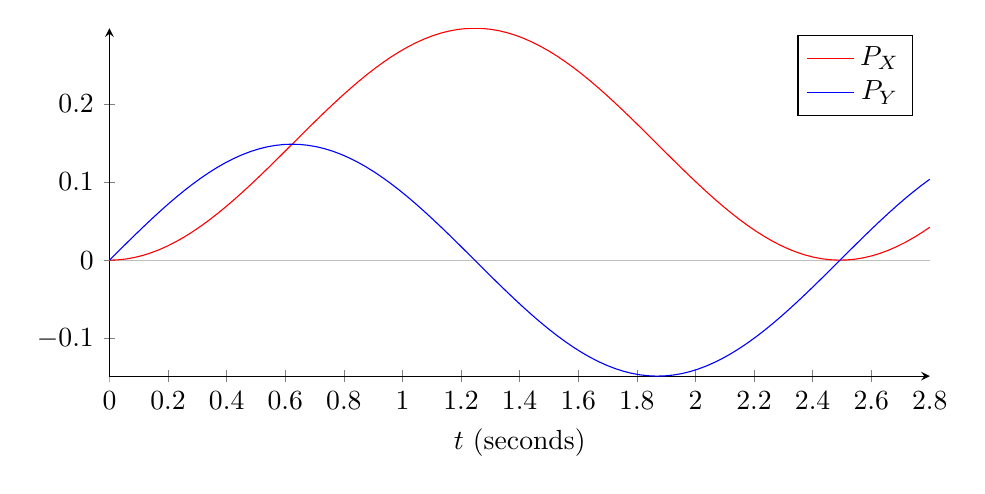
\begin{tikzpicture}
        \begin{axis}[
            width = 12cm,
            height = 6cm,
            axis lines = left,
            xlabel = {$t$ (seconds)},
            extra y ticks = 0,
            extra y tick labels = ,
            extra y tick style = { grid = major },
        ]
        \addplot [
            domain=0:2.8, 
            samples=100, 
            color=red,
        ] {(0.374 / 2.52) * (1 - cos(deg(2.52 * x)))};
        \addlegendentry{$P_X$}
        \addplot [
            domain=0:2.8, 
            samples=100, 
            color=blue,
        ] {(0.374 / 2.52) * sin(deg(2.52 * x))};
        \addlegendentry{$P_Y$}
        \end{axis}
    \end{tikzpicture}
    \caption{The yaw $P_X$ and pitch $P_Y$ of a tight spiral pass as functions of time, with parameters given by equation \ref{parameters} and initial attitudes $P_X = 0$ and $P_Y = 0$.}
    \label{P vs time}
\end{figure}
Note that the pitch of the football $P_Y$ follows a sine wave, so it periodically intersects $0$. This is the resolution to our paradox! Because the ball always returns to zero pitch relative to its velocity, it appears to the viewer as if the orientation of the ball's longitudinal axis follows its trajectory. Thus, when the football descends, we see its nose dip as its pitch compensates for its downward velocity.

We can visualize this behavior in perhaps a more intuitive manner by graphing $P_X$ and $P_Y$ parametrically, which yields figure \ref{P parametric}.

\begin{figure}[h!]
    \centering
    \begin{tikzpicture}
        \begin{axis}[
            width = 10cm,
            height = 10cm,
            axis lines = middle,
            axis equal,
            xmin = -0.4,
            xmax = 0.4,
            xlabel = {$P_X$},
            xticklabel style={/pgf/number format/fixed},
            ylabel = {$P_Y$},
            yticklabel style={/pgf/number format/fixed}
        ]
        \addplot [
            domain=0:2.49332750285, 
            samples=100, 
            color=green,
        ] ({(0.374 / 2.52) * (1 - cos(deg(2.52 * x)))}, {(0.374 / 2.52) * sin(deg(2.52 * x))});
        \end{axis}
    \end{tikzpicture}
    \caption{The path of the deviation vector $\mathbf{P}$ with initial attitudes $P_X = 0$ and $P_Y = 0$.}
    \label{P parametric}
\end{figure}
Figure \ref{P parametric} can be thought of as showing the yaw and pitch of the ball from the perspective of the quarterback, as opposed to figure \ref{projection}, which shows $\mathbf{P}$ from roughly the perspective of the receiver. $\mathbf{P}$ starts at $(0, 0)$, but proceeds clockwise following a circular path throughout the ball's flight. This confirms our theory that the ball gyroscopically precesses; in our case, the nose of the spiral is akin to the tip of the top in figure \ref{top2}.

Furthermore, figures \ref{precession} introduce the idea that the greater $\mathbf{\hat{d}}$ is in the $+z$ direction, the stronger the torque on the ball in the $-y$ direction. Figure \ref{P parametric} reflects this idea in that the greater $P_X$ is in the $\mathbf{\hat{X}}$ direction, the faster $P_Y$ decreases in the $\mathbf{\hat{Y}}$ direction due to torque, creating the clockwise path shown. It follows that because $P_X$ is always positive, the torque on the ball is often in the $-y$ direction, allowing the ball's longitudinal axis to keep up with its velocity's downward rotation.

In simplest terms, the angle of a spiraling football follows its trajectory because $P_Y$ regularly returns to $0$.

\section{Conclusion}
Without gravity, the so-called paradox described in this article would not exist. Even when taking gravity and air resistance into account, a physicist who has never watch football would probably not predict that a spiral pass would maintain tangency with its trajectory. Physics, however, is often counterintuitive. 

By causing the ball's velocity to dip, gravity sets off a chain reaction in which air resistance causes a torque on the ball, which causes the ball's angular momentum to rotate, which causes the ball to wobble, which causes the ball's longitudinal axis to dip with its velocity, creating an easier pass for the receiver. So next time you see a deep spiral touchdown pass on TV, try to spot the wobble in the slow motion replay. Without that wobble, those 6 points may not be on the board.

\nocite{*}
\printbibliography

\end{document}